\documentclass{article}

\usepackage[letterpaper,top=2.5cm,bottom=2.5cm,left=2.5cm,right=2.5cm]{geometry}
\usepackage{amsmath,amssymb,amsthm}
\usepackage{graphicx}
\usepackage{hyperref}
\usepackage{cleveref}
\usepackage{xcolor}

\newtheorem{theorem}{Theorem}
\newtheorem{lemma}{Lemma}
\newtheorem{corollary}{Corollary}
\newtheorem{conjecture}{Conjecture}

\newcommand{\matias}[1]{\textcolor{red}{#1}}
\newcommand{\RR}{\mathbb{R}}
\setlength{\emergencystretch}{1em}

\title{A Hadamard matrix with growth factor greater than its order}
\author{Matias Andia\thanks{Department of Mathematics, Princeton University,
Princeton, NJ. \texttt{mati@princeton.edu}}}
\date{}

\begin{document}
\maketitle

\begin{abstract}
It has long been conjectured that the growth factor of a completely pivoted
Hadamard matrix is equal to its order. In this paper, we construct a row and
column permutation of the Sylvester Hadamard matrix of order $4096$ that is
completely pivoted and has growth factor $4608=(9/8)4096$, disproving the conjecture. This construction extends to give a completely pivoted Hadamard matrix of order $2^d$ with growth factor $(9/8)2^d$ for every integer $d\ge12$.
\end{abstract}

\section{Introduction}\label{sec:introduction}
A matrix $H\in\RR^{n\times n}$ is a Hadamard matrix of order $n$ if its
entries are $\pm1$ and $HH^\top=nI$. We say that $H$ is \emph{completely pivoted} (CP) if, at every step of Gaussian elimination without row or column interchanges, the pivot has maximum absolute value among the entries of the current Schur complement. Write $p_k$ for the magnitude
of the $k$-th pivot. The growth factor is the largest entry magnitude
encountered during elimination, divided by the largest entry magnitude of
the original matrix. For a CP Hadamard matrix, it is therefore
\[
       g(H)=\max_{1\le k\le n}p_k.
\]

For a CP Hadamard matrix $H$ of order $n$, the final pivot has magnitude $n$, so $g(H)\ge n$. A long-standing conjecture asserts that equality always holds~\cite{Cryer,DP}. Equivalently, the conjecture states that no earlier pivot
can exceed the final one in magnitude. Much of the previous
work on this question has focused on the possible pivot sequences of CP Hadamard matrices (see, e.g.,
Day and Peterson~\cite{DP} and Edelman and
Friedman~\cite{EF}). For a broader discussion of growth factors under complete pivoting, see Edelman and Urschel~\cite{EU}.

We construct a counterexample by permuting the rows and columns of a Sylvester Hadamard matrix. For
$n=2^d$, let $W_n$ be the Sylvester matrix, defined by
\[
 W_1=(1),\qquad
 W_{2n}=\begin{pmatrix}W_n&W_n\\W_n&-W_n\end{pmatrix}.
\]

\begin{theorem}\label{thm:main}
There are permutation matrices $P,Q$ for which
$H=PW_{4096}Q$ is completely pivoted and
\[
       g(H)=p_{4089}=4608=\frac{9}{8}4096.
\]
\end{theorem}


Our permutations allow us to reach a $14\times14$ Schur complement with entries $\pm n/4$.
Six further eliminations produce an entry of magnitude $9n/8$.
The matrix is shown in \Cref{fig:matrix}.

\section{Construction and verification}\label{sec:construction}

We now describe the construction of the completely pivoted ordering in
\Cref{thm:main}. The main idea is to begin with a short pivot sequence on a
small Sylvester matrix, lift it to a larger matrix, and continue elimination
on the remaining Schur complement. We repeat this procedure until the desired
pivot appears.

\subsection{Lifting a pivot sequence}\label{sec:lifting}
The following lemma formalizes the lifting step described above. It is a version of an observation due to Tornheim and is given in Peca-Medlin~\cite[Proposition 2.10]{PM}.
We include a proof for completeness.


\begin{lemma}\label{lem:lift}
Suppose $S$ is a matrix whose upper-left entry $p=S_{11}\ne0$
is a complete pivot, so that $|p|=\|S\|_{\max}$. Then the first two pivots of $S\otimes W_2$ are complete pivots, with values $p$ and $-2p$. After these two steps, the remaining Schur complement is the Schur complement of $S$ after eliminating $p$, tensored with $W_2$.
\end{lemma}

\begin{proof}
The first pivot $p$ of $S\otimes W_2$ is indeed a complete pivot because
$\|S\otimes W_2\|_{\max}=|p|$. After this elimination, every entry of the resulting Schur complement has magnitude at most $2|p|$, while its upper-left entry is $-p-p^2/p=-2p$. Thus, the second pivot is also a complete pivot.

The two steps together eliminate the upper-left $2\times2$ block $pW_2$ of $S\otimes W_2$. Therefore, for $i,j>1$, the
corresponding block of the remaining Schur complement is
\[
S_{ij}W_2-(S_{i1}W_2)(pW_2)^{-1}(S_{1j}W_2)
=\left(S_{ij}-\frac{S_{i1}S_{1j}}{p}\right)W_2,
\]
the claimed tensor-product Schur complement.
\end{proof}

Using the fact that $W_{2n}=W_n\otimes W_2$, applying this lemma twice, gives that any sequence of $k$ complete pivots on $S$ lifts to a sequence of $4k$ complete pivots on $S\otimes W_4$. Moreover, the Schur complement remaining after the lifted sequence is the original remaining Schur complement tensored with $W_4$. This allows us to lift an initial complete-pivoting sequence on $W_n$ to one on $W_{4n}$.

\subsection{The five stages}\label{sec:five-stages}

We start with $W_{16}$ and choose ten complete pivots, leaving a
$6\times6$ Schur complement with entries $\pm4$. After lifting the sequence
to $W_{64}$, the remaining Schur complement has order $24$. We then choose
sixteen more pivots so that the resulting $8\times8$ Schur complement has
entries $\pm16$. Repeating these steps gives the five stages shown in
\Cref{fig:construction}. At each stage, the entries of the final Schur
complement have magnitude $n/4$, while its order increases by two.

The lifting lemma determines the pivots in each lifted sequence, so only the additional choices made in the smaller Schur complements need to be checked directly. These choices were found computationally by searching among the entries of largest magnitude in the current Schur complement. We perform the Schur updates in rational arithmetic and verify that each selected pivot has maximum absolute value in the current matrix.

Thus, for $n=4096$, the first $n-14=4082$ complete pivoting steps leave a Schur complement $(n/4)K$, where $K$ is a particular $14\times14$ sign matrix. To obtain a pivot exceeding $n$, it remains to show that complete pivoting on $K$ produces a pivot of magnitude greater than $4$.

\begin{figure}[htbp]
\centering
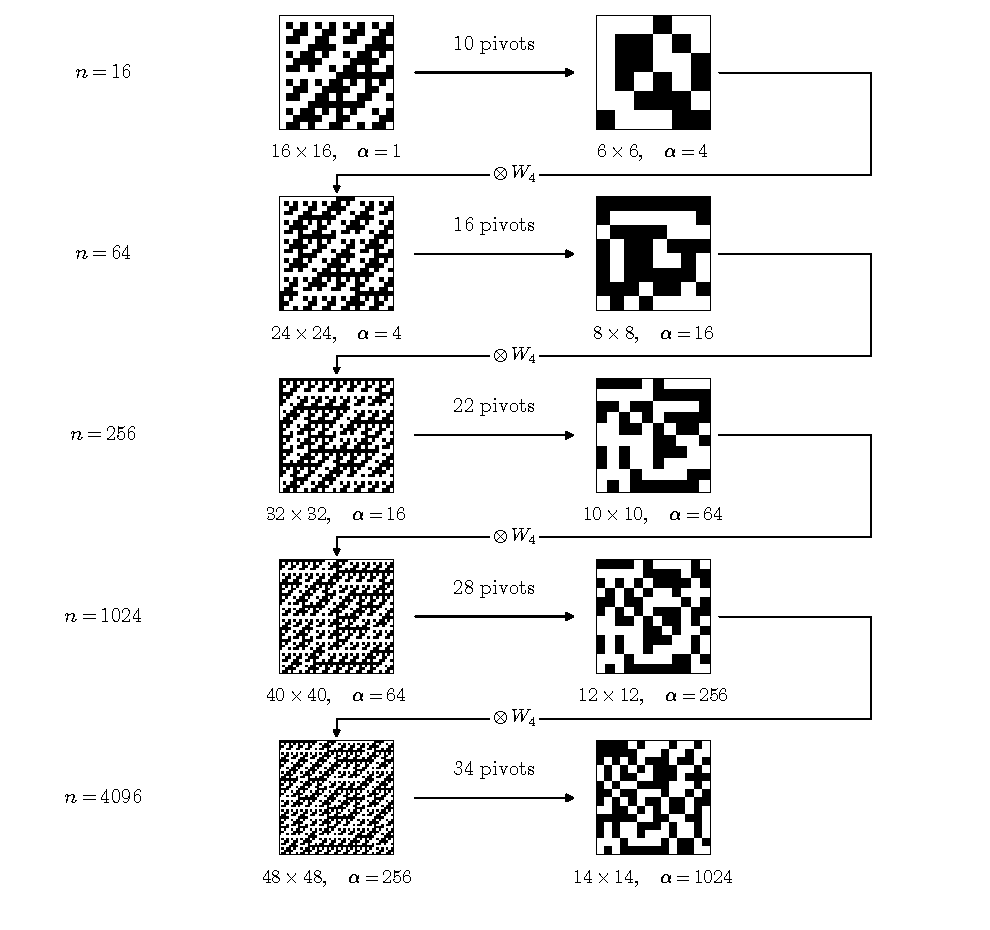
\includegraphics[width=0.95\textwidth]{figures/construction.pdf}
\caption{The five stages of the construction. Each square shows a Schur
complement divided by its entry magnitude $\alpha$. Black entries are $-1$ and white entries are $+1$.}
\label{fig:construction}
\end{figure}
\subsection{The pivot exceeding the order}\label{sec:large-pivot}
Continuing complete pivoting on $(n/4)K$ gives the final fourteen pivot magnitudes
\begin{align}\label{eq:last}
    (p_{n-13},\ldots,p_n)
    =\frac n4\left(1,2,2,2,4,4,\frac92,\frac{10}{9},
        \frac65,\frac43,1,2,2,4\right).
\end{align}
In particular, the seventh pivot in this sequence has magnitude $9n/8$.
Explicitly, after six
eliminations on $(n/4)K$, we obtain
\begin{align*}
\frac n8
\begin{pmatrix}
 9&-5&-4&7&-3&-2&-1&-1\\
 -4&0&0&-4&0&0&0&0\\
 3&-3&0&1&-1&-2&1&1\\
 -1&1&0&-3&-1&2&1&1\\
 -2&2&0&-2&2&0&2&-2\\
 1&-1&0&-1&1&2&-1&-1\\
 -2&2&0&-2&2&0&-2&2\\
 -4&4&4&-4&0&0&0&0
\end{pmatrix}.
\end{align*}
The maximum absolute entry of this matrix is the top-left entry $9n/8$.
It is therefore a valid complete pivot, namely $p_{n-7}=9n/8$.

\begin{proof}[Proof of \Cref{thm:main}]
The construction above, together with \Cref{lem:lift}, gives
a sequence of complete pivots for $W_{4096}$.
By applying the corresponding row and column permutations in advance, we obtain a completely pivoted matrix
$H=PW_{4096}Q$.

Since row and column permutations preserve the orthogonality of $W_{4096}$, $H$ is Hadamard. The pivots before the final
fourteen steps have magnitude at most $1024$, while \eqref{eq:last} shows that the largest of the remaining
pivots is $p_{4089}=4608$. Hence
\[
    g(H)=p_{4089}=4608=\frac98\,4096.
\]
\end{proof}
\section{Larger orders and asymptotic growth}\label{sec:larger-orders}

The lifting argument also shows that this counterexample extends to all orders $2^d$ with $d\ge12$.

\begin{corollary}\label{cor:family}
For every integer $d\ge12$, there exists a completely pivoted row and column
permutation of $W_{2^d}$ whose growth factor is $(9/8)2^d$.
\end{corollary}

\begin{proof}
Let $H$ be completely pivoted. By \Cref{lem:lift}, we can choose an ordering
of $H\otimes W_2$ that is completely pivoted and satisfies
\begin{align*}
    g(H\otimes W_2)=2g(H).
\end{align*}
Starting with the matrix $H$ from \Cref{thm:main} and applying this construction
repeatedly proves the result.
\end{proof}

We can express this result in terms of the largest possible growth factor
among completely pivoted Hadamard matrices of a given order. For any $n$ for
which a Hadamard matrix exists, define
\[
    \Gamma_{\mathrm{Had}}(n)
    :=\max\{g(H):H\text{ is a CP Hadamard matrix of order }n\}.
\]
By \Cref{cor:family},
we have
\begin{align*}
    \Gamma_{\mathrm{Had}}(2^d)\ge\frac98\,2^d,\qquad d\ge12.
\end{align*}

Shah and Urschel~\cite{SU} showed that the largest growth factor under
complete pivoting for arbitrary real matrices is $n^{\Theta(\log n)}$. Combined with the restricted-entry result of Edelman and Urschel~\cite[Theorem~3.3]{EU}, this implies the same asymptotic behavior for sign matrices. We conjecture that imposing the additional requirement of orthogonality, thereby restricting to Hadamard matrices, does not change this asymptotic behavior.

\begin{conjecture}\label{conj:asymptotic}
As $n\to\infty$ through the orders for which Hadamard matrices exist,
\begin{align*}
    \Gamma_{\mathrm{Had}}(n)=n^{\Theta(\log n)}.
\end{align*}
\end{conjecture}
Although Sylvester's construction gives Hadamard matrices of arbitrarily large order, it remains unknown whether a Hadamard matrix exists at every order divisible by four (the classical Hadamard conjecture~\cite{HW}). Thus, even the set of orders for which $\Gamma_{\text{Had}}(n)$ is defined is not fully understood.

The upper bound already follows from the general complete pivoting bound.
Thus the conjecture asserts that there is a constant $c>0$ such that
$\Gamma_{\mathrm{Had}}(n)\ge n^{c\log n}$ for all sufficiently large Hadamard
orders $n$. Since in our lifting construction the ratio $g(H)/n$ is constant, it does not give a lower bound.

\paragraph{Acknowledgements.}
AI tools were used extensively in constructing this counterexample. In particular, GPT-6 Astra Pro produced the counterexample after a long exploration into this conjecture. Selected prompts and conversation excerpts from this exploration, together with scripts for verifying all computational results, are available at \url{https://github.com/matias-ma/hadamard_cp}. The author organized the final presentation and takes full responsibility for all content. 


\bibliographystyle{plain}
\bibliography{citations}

\begin{figure}[p]
\centering
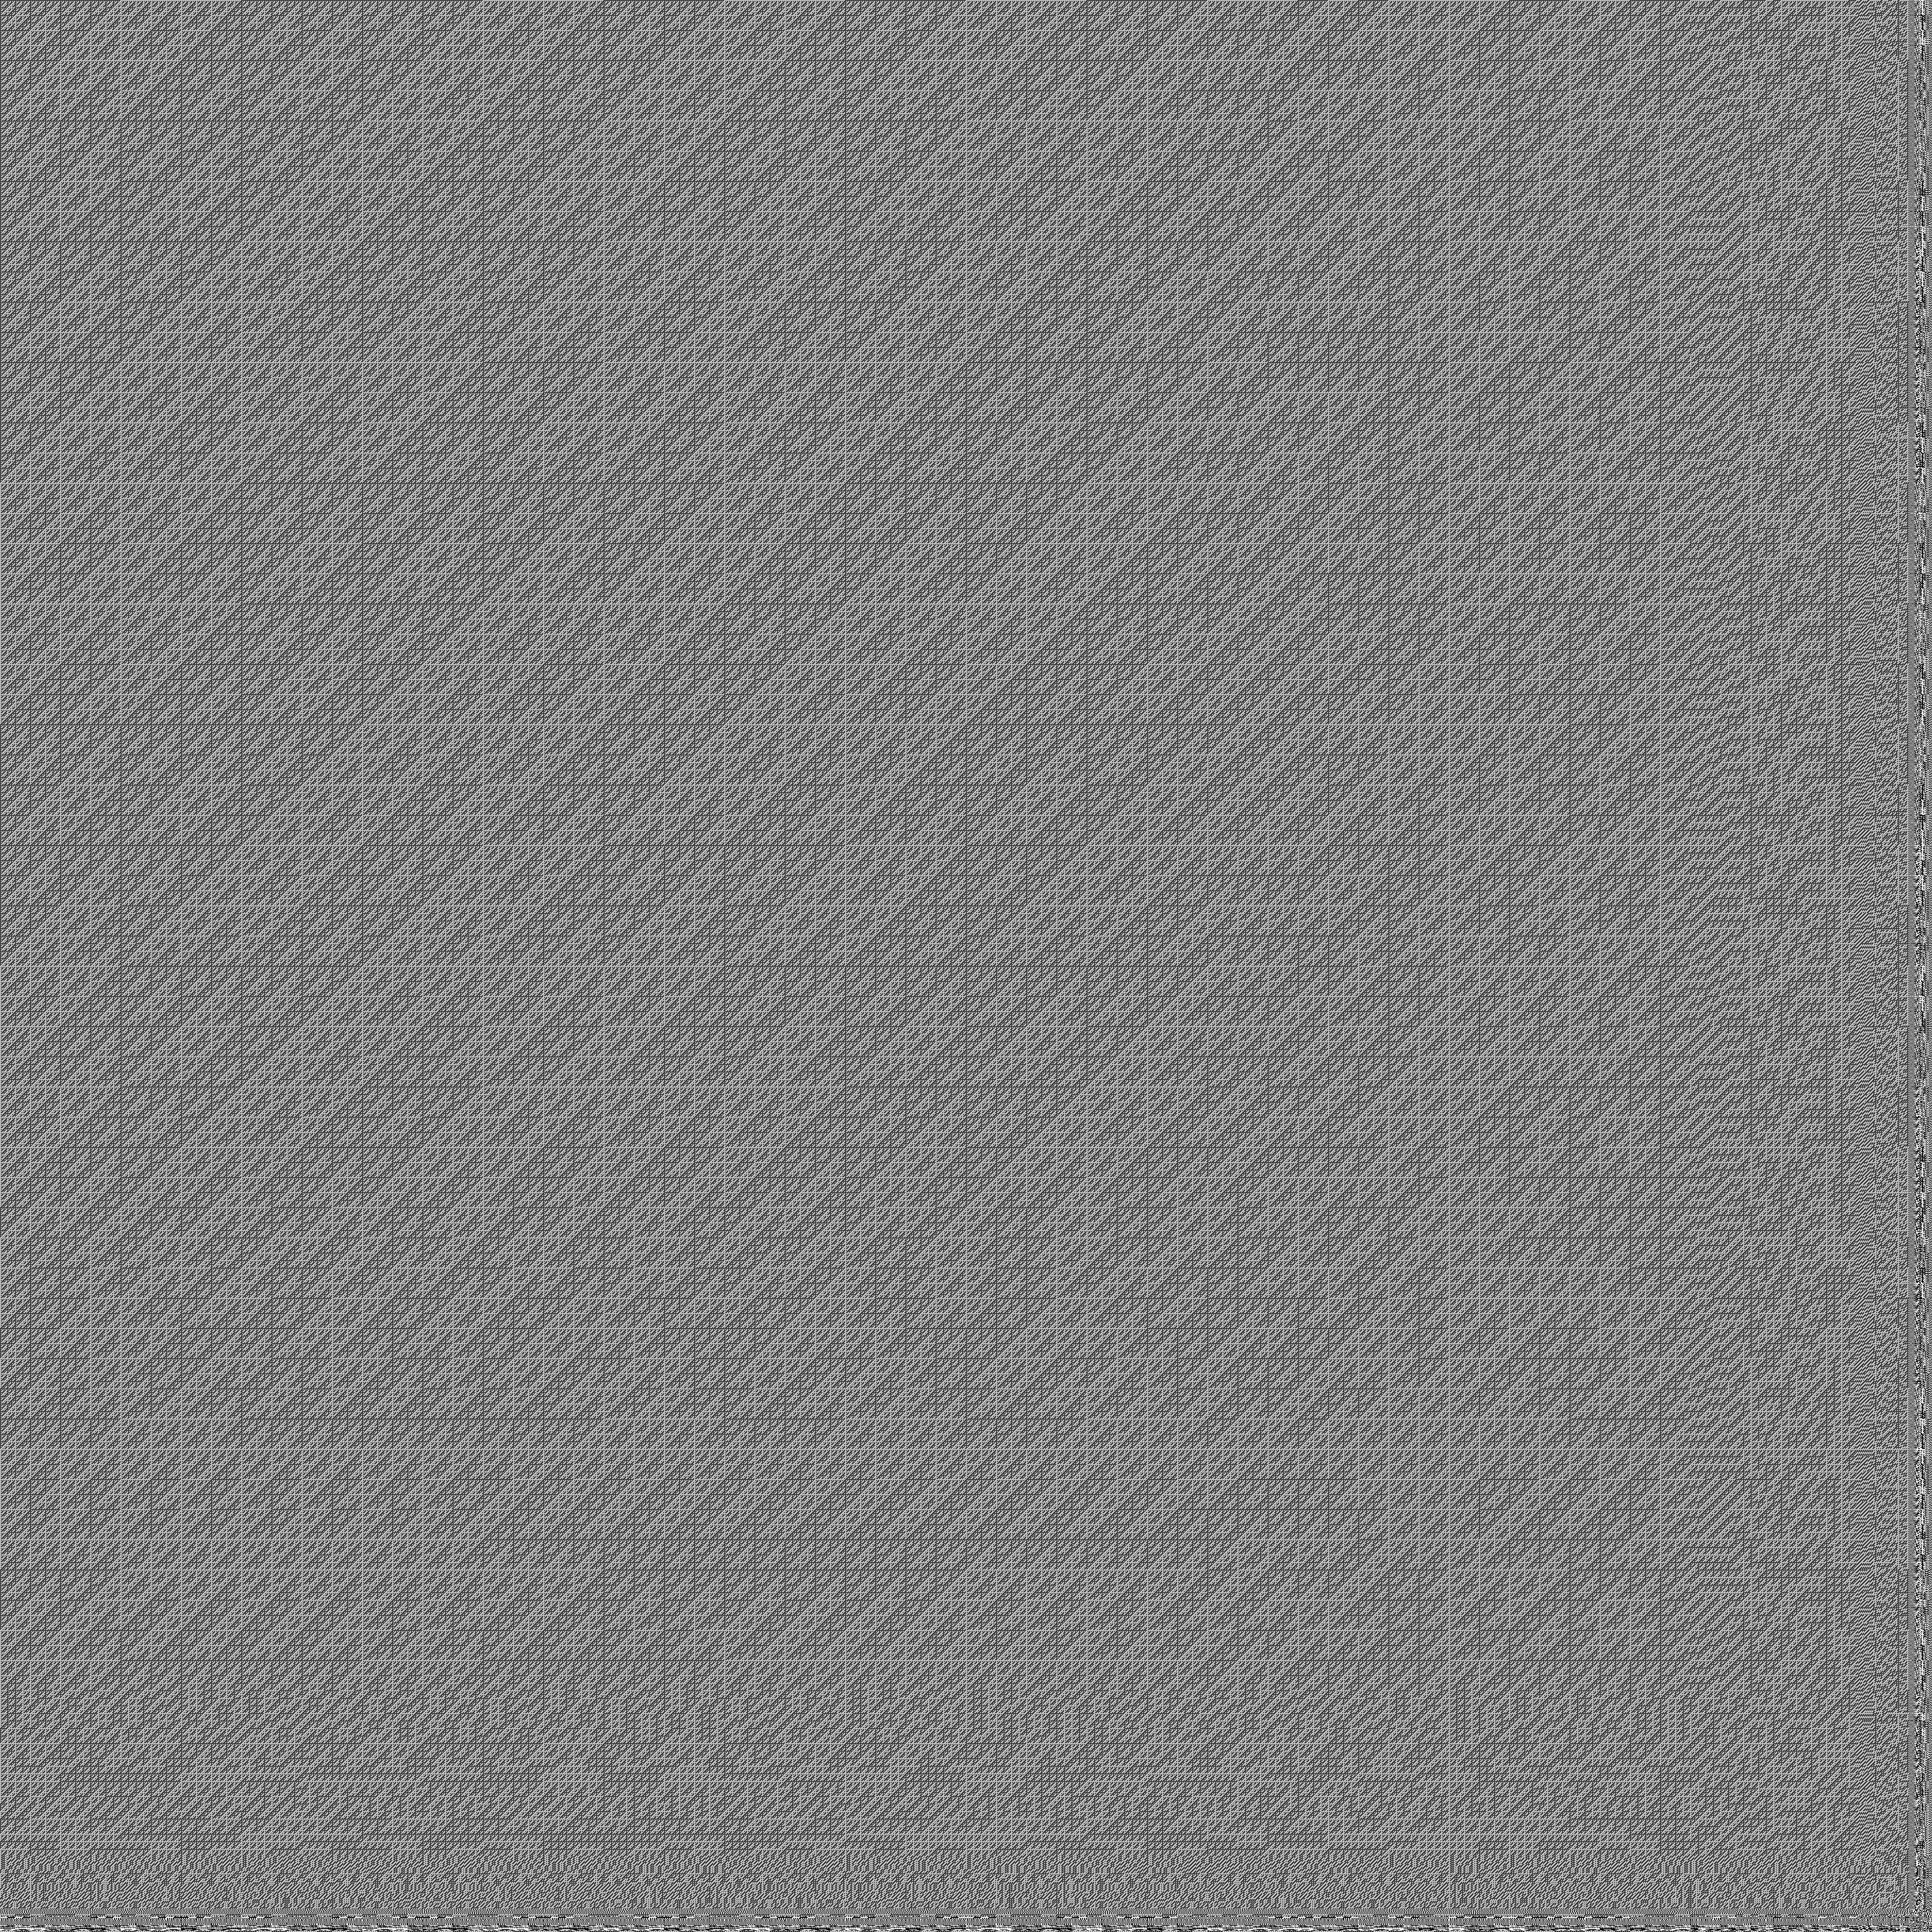
\includegraphics[width=1\textwidth]{figures/matrix.png}
\caption{The completely pivoted $4096\times4096$ Hadamard matrix $H$ from
\Cref{thm:main}. Black denotes $-1$ and white denotes $+1$. Each pixel represents one entry.}
\label{fig:matrix}
\end{figure}

\end{document}
